\documentclass [12pt, a4paper]{article}

%Includes 
\usepackage[utf8]{inputenc}
\usepackage{graphicx}
\usepackage{subfig}
\usepackage[spanish]{babel}
\graphicspath{{images/}}
\usepackage{imakeidx}
\usepackage{enumerate}
\usepackage{listings} 

% Inicio de documento
\title{UNIVERSIDAD DE BUENOS AIRES\\FIUBA\\
	\vspace{10mm}
\includegraphics[scale=0.4]{fiuba}
	\vspace{5mm}\\66.20 Organización de Computadoras\\
	Trabajo práctico 0: Infraestructura básica\\1$^{er}$ cuatrimestre de 2018}

\author{ \textbf{ALUMNOS} 
	\vspace{5mm}\\
	\textbf{92454 ZARAGOZA, MARTIN}\\
	\textbf{92691 SIBIKOWSKI, NICOLAS}\\
	\textbf{91985 DUFAU, EZEQUIEL}\\
}
\date{}
\makeindex[columns=1, title=Indice, intoc]
\setlength{\parindent}{12pt}


\begin{document}


	\lstset{language=C}  
	\maketitle
	
	\clearpage
	\section{\index{Introducción}Introdución}
	Este documento representa la documentación técnica  del trabajo práctico 0, correspondiente a la materia \textbf{66.20 Organización de Computadoras}\\
	En el mismo se incluira el desarrollo de los siguientes puntos:
		\begin{itemize}
			\item Diseño e Implementación
			\item Compilación y ejecución del programa
			\item Corridas de prueba
			\item Código Fuente
		\end{itemize}
	\section{\index{Diseño e Implemantación}Diseño e Implementación} 
	Se desarrolló un programa que permite dibujar el conjunto de Julia, en lenguaje C.
	
	\subsection{Tipos de Datos Abstractos}
	Se diseñaron los siguientes TDAs:
	\subsubsection{\textbf{Pixel}}
		Define un punto en el plano complejo
	\begin{lstlisting}[frame=single]
typedef struct {
unsigned x;
unsigned y;
} Pixel;

typedef struct {
unsigned width;
unsigned height;  
} Dimension;

typedef Dimension Resolution;

void parseRes(char* str , Resolution* targetRes);

#endif
		
	\end{lstlisting}
	
	\vspace{5mm}
	\subsubsection{\textbf{Complex}}
		Define el TDA para manejar números complejos
	\begin{lstlisting}[frame=single]
typedef struct {
double re;
double im;
} Complex;

typedef struct {
double left;
double right;
double top;
double bottom;
} Boundaries;

Complex newCpx(double re , double im);

/** 
* Obtiene un numero complejo a partir de un string
*/
void parseCpx(char* str , Complex* targetCpx);

/**
* Obtiene la raiz cuadrada de un complejo
*/
Complex pow2Cpx(Complex* value);

Complex addCpx(Complex* first , Complex* second);

/** 
* Obtiene el modulo de un valor complejo 
  (distancia respecto al origen).
*/
double modCpx(Complex* value);

/** 
* Calcula los limites del plano complejo 
   (el rectangulo a mapear del plano complejo).
* Dimension dim - Tamano del plano complejo
* Complex center - Valor de centro EN EL plano
*/
Boundaries getBoundaries(Complex* dim , Complex* center);

#endif

	\end{lstlisting}
	
	
	\clearpage
	\section{\index{Compilación y ejecución del programa}Compilación y ejecución del programa}
	
	Utilizamos el programa GXemul para simular un entorno de desarrollo. El mismo consta de una máquina MIPS corriendo una versión del sistema operativo BSD. Debido a esto, el compilador utilizado utilizado es el que trae instalada la imagen provista por la cátedra. El mismo es el \textbf{(GCC) 3.3.3 (NetBSD nb3 20040520)}
	\\\\
	Para facilitar el proceso de compilación, programamos un Makefile, seteando las opciones correspondientes. Se debe ejecutar make en el directorio raiz del proyecto y el programa queda compilado. Se genera un ejecutable llamado app.exe. 
	
	\section{\index{Corridas de prueba}Corridas de prueba}
	\subsection{Valores por defecto}
	Se generó un dibujo usando los valores por defecto, barriendo la región rectangular del plano comprendida entre los vértices -2+2i y+2-2i.	La validación fue visual. Comparando contra un dibujo patrón disponible en el enunciado.
	
	\paragraph{Comando ejecutado: tp0 -o uno.pgm }
	
	Resultado de la prueba:
	\begin{figure}[h]
		\centering
		\subfloat[nuestro programa]{
			\label{f:nuestro}
			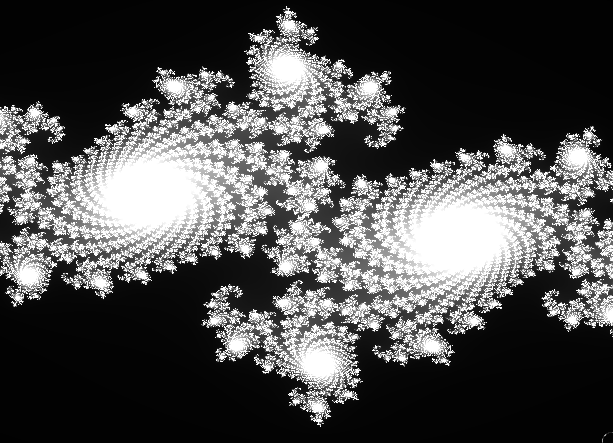
\includegraphics[width=0.3\textwidth]{uno.png}}
		\subfloat[trabajo práctico]{
			\label{f:tp}
			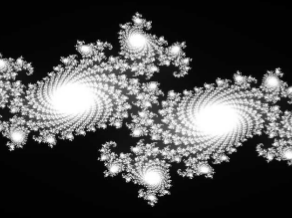
\includegraphics[width=0.3\textwidth]{unoTp}}
		\caption{Comparación entre imagen generada por el enunciado del tp, y nuestro programa}
		\label{f:comparacion1}
	\end{figure}
	\subsection{Zoom en región}
	Hacemos zoom sobre la región centrada en 0.282-0.007i, usando un
	rectángulo de 0.005 unidades de lado.
	
	\paragraph{Comando ejecutado: tp0 -c 0.282-0.007i -w 0.005 -H 0.005 -o dos.pgm}
	
	Resultado de la prueba:
	\begin{figure}[h]
		\centering
		\subfloat[nuestro programa]{
			\label{f:nuestro}
			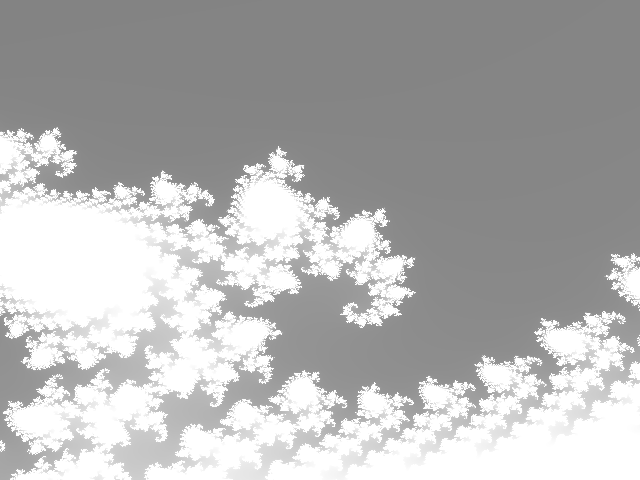
\includegraphics[width=0.3\textwidth]{dos}}
		\subfloat[enunciado del trabajo práctico]{
			\label{f:tp}
			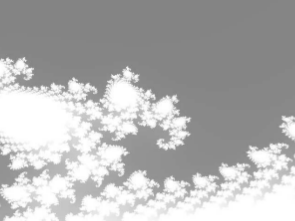
\includegraphics[width=0.3\textwidth]{dosTp}}
		\caption{Comparación entre la imagen generada por el enunciado del tp, y nuestro programa}
		\label{f:comparacion2}
	\end{figure}

	\subsection{Modificación de la semilla}
	En está prueba vamos a modificar la semilla utilizando el comando -s. Apoyandonos mediante otra implementación del Algoritmo de Julia, vamos a comparar la imagen generada por nuestro programa coon la generada por la otra implementación.
	
	Resultado de la prueba:
		\begin{figure}[h]
		\centering
		\subfloat[nuestro programa]{
			\label{f:nuestro}
			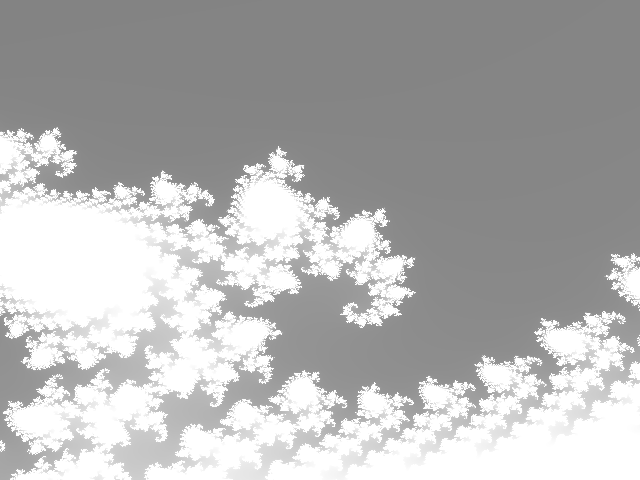
\includegraphics[width=0.3\textwidth]{dos}}
		\subfloat[enunciado del trabajo práctico]{
			\label{f:tp}
			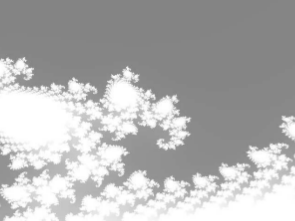
\includegraphics[width=0.3\textwidth]{dosTp}}
		\caption{Comparación entre otra implementación del algoritmo de Julia y nuestro programa}
		\label{f:comparacion3}
	\end{figure}
	\printindex
\end{document}
